\title{Aula 7 - Circuitos e Portas Lógicas}



\begin{frame}
    \titlepage
\end{frame}

% --- 1. INTRODUÇÃO E CONCEITOS ---

\begin{frame}{Sistema Binário e Lógica Booleana}
    \begin{itemize}
        \item \textbf{Sistema Binário:} Utiliza apenas dois dígitos (1 e 0), representados por faixas de tensão, ideais para representar relações lógicas.
        \item \textbf{Lógica Booleana:} Desenvolvida por George Boole (1854), baseia-se na tomada de decisões lógicas sobre circunstâncias verdadeiras ou falsas.
        \item \textbf{Álgebra Booleana:} Sistema que emprega símbolos (como A, B e C) e operadores para representar expressões lógicas, simplificando a notação.
    \end{itemize}
\end{frame}

\begin{frame}{Estados Lógicos e Abstração}
    \begin{itemize}
        \item \textbf{O que são Estados Lógicos?}
              \begin{itemize}
                  \item Representações de condições que assumem apenas \textbf{dois valores possíveis}: ou é uma coisa, ou é outra.
              \end{itemize}

        \item \textbf{Exemplos do cotidiano:}
              \begin{itemize}
                  \item Lâmpada: Acesa \textit{ou} Apagada
                  \item Condição: Vivo \textit{ou} Morto
                  \item Evento: Aconteceu \textit{ou} Não aconteceu
                  \item Existência: Existe \textit{ou} Não existe
              \end{itemize}

        \item \textbf{Tradução Tecnológica:}
              \begin{itemize}
                  \item \textbf{Álgebra Booleana:} Traduz situações para valores Verdadeiro (\textit{True}) ou Falso (\textit{False}).
                  \item \textbf{Eletrônica Digital:} Lê estados como níveis de tensão (Binário 1 e Binário 0).
              \end{itemize}
    \end{itemize}
\end{frame}

% --- 2. FUNDAMENTOS MATEMÁTICOS ---

\begin{frame}{Álgebra Booleana vs. Convencional}
    \begin{itemize}
        \item \textbf{Diferença Principal:} Na álgebra booleana, constantes e variáveis podem ter apenas dois valores possíveis: \textbf{0} ou \textbf{1}.
        \item \textbf{Natureza das Variáveis:} Não representam números efetivos, mas o estado do \textbf{nível lógico} de uma tensão.
        \item \textbf{Simplicidade:} Não existem frações, decimais, números negativos, logaritmos ou números imaginários.
    \end{itemize}
\end{frame}

\begin{frame}{Variáveis na Álgebra Booleana}
    \begin{itemize}
        \item \textbf{Definição:} Modo de expressar a relação entre as entradas e as saídas de um circuito lógico.
        \item \textbf{Representação:} Usamos letras (ex: $A, B, C$) para representar as variáveis.
        \item \textbf{Dualidade:} Em um instante qualquer, $A = 0$ ou $A = 1$. Se não for um valor, será obrigatoriamente o outro.
    \end{itemize}
\end{frame}

% --- 3. IMPLEMENTAÇÃO FÍSICA E NÍVEIS ---

\begin{frame}{Níveis de Tensão e Faixas de Operação}
    Em um sistema digital, o valor lógico é determinado pela tensão medida:
    \begin{itemize}
        \item \textbf{Nível Lógico 0:} Qualquer tensão entre $0$ e $0,8$ V.
        \item \textbf{Nível Lógico 1:} Qualquer tensão entre $2$ e $5$ V.
    \end{itemize}
    \vspace{0.3cm}
    \begin{block}{Observação Importante}
        Tensões entre $0,8$ V e $2$ V são consideradas \textbf{indefinidas} e não devem ocorrer em circunstâncias normais de operação.
    \end{block}
\end{frame}

\begin{frame}{Termos Sinônimos para Níveis Lógicos}
    Os níveis 0 e 1 são referenciados por diversos termos (Tabela 3.1):
    \vspace{0.2cm}
    \begin{table}
        \small
        \centering
        \begin{tabular}{cc}
            \hline
            \textbf{Nível Lógico 0} & \textbf{Nível Lógico 1} \\ \hline
            Falso                   & Verdadeiro              \\
            Desativado (OFF)        & Ativado (ON)            \\
            Baixo (LOW)             & Alto (HIGH)             \\
            Não                     & Sim                     \\
            Aberto                  & Fechado                 \\
            Apagado                 & Aceso                   \\
            Morto                   & Vivo                    \\
            Não aconteceu           & Aconteceu               \\
            Inexistente             & Existente               \\ \hline
        \end{tabular}
    \end{table}
\end{frame}

% --- 4. OPERAÇÕES E CIRCUITOS ---

\begin{frame}{Operações Lógicas Básicas}
    A álgebra booleana possui apenas três operações fundamentais:
    \vspace{0.4cm}
    \begin{enumerate}
        \item \textbf{OR (OU)}
        \item \textbf{AND (E)}
        \item \textbf{NOT (NÃO)}
    \end{enumerate}
    \vspace{0.4cm}
    \begin{block}{Portas Lógicas}
        Circuitos digitais (com diodos, transistores e resistores) que realizam essas operações básicas sobre as entradas para gerar uma saída.
    \end{block}
\end{frame}

\begin{frame}{Circuitos Lógicos e Aplicações}
    \begin{itemize}
        \item \textbf{Portas Lógicas:} São os blocos fundamentais de todos os circuitos e sistemas digitais.
        \item \textbf{Análise e Simplificação:} A álgebra permite reescrever circuitos utilizando menos portas e conexões.
        \item \textbf{Síntese:} Atua como ferramenta de projeto para criar relações específicas entre entrada e saída.
    \end{itemize}
\end{frame}

\begin{frame}{Finalidades da Álgebra Booleana}
    A álgebra booleana é utilizada para dois objetivos principais:
    \begin{itemize}
        \item \textbf{Descrição e Análise:} Entender o funcionamento individual das portas lógicas básicas.
        \item \textbf{Projeto:} Analisar e projetar circuitos combinacionais complexos a partir da união dessas portas.
    \end{itemize}
\end{frame}


\begin{frame}{Tabelas-Verdade: Conceito}
    \begin{itemize}
        \item \textbf{Definição:} Técnica para descrever como a saída de um circuito lógico depende dos níveis lógicos presentes em suas entradas.
        \item \textbf{Estrutura:}
              \begin{itemize}
                  \item \textbf{Lado Esquerdo:} Lista todas as combinações possíveis das entradas ($A, B, C \dots$).
                  \item \textbf{Lado Direito:} Indica o nível lógico resultante na saída ($x$) para cada combinação.
              \end{itemize}
        \item \textbf{Funcionamento:} Cada linha representa um estado específico do sistema. Se as entradas mudam, a saída segue o valor definido na linha correspondente.
    \end{itemize}
\end{frame}

\begin{frame}{Tabelas Verdade}

    \begin{figure}
        \centering

        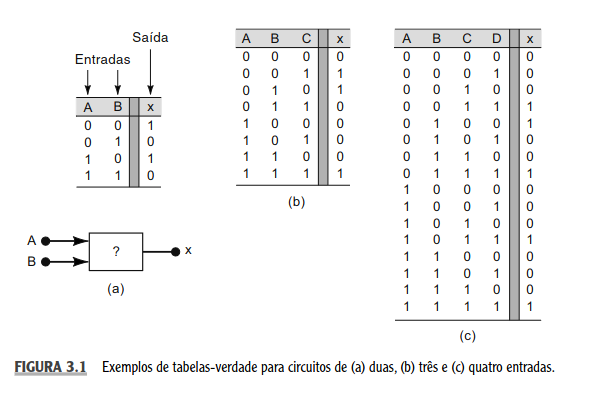
\includegraphics[width=\textwidth]{Figuras/TabelaVerdade.png}

    \end{figure}

\end{frame}

\begin{frame}{Número de Combinações}
    O número de linhas de uma tabela-verdade depende da quantidade de entradas ($N$):
    \vspace{0.3cm}
    \begin{block}{Regra Exponencial}
        O número de combinações de entrada é igual a $2^N$.
    \end{block}
    \vspace{0.3cm}
    \begin{itemize}
        \item \textbf{2 entradas:} $2^2 = 4$ combinações (linhas).
        \item \textbf{3 entradas:} $2^3 = 8$ combinações (linhas).
        \item \textbf{4 entradas:} $2^4 = 16$ combinações (linhas).
    \end{itemize}
\end{frame}

\begin{frame}{Organização e Contagem Binária}

    \begin{itemize}
        \item \textbf{Preenchimento:} Para não esquecer nenhuma combinação, as entradas são listadas em \textbf{sequência de contagem binária}.
        \item \textbf{Exemplo (2 entradas):}
              \begin{itemize}
                  \item 00 (zero)
                  \item 01 (um)
                  \item 10 (dois)
                  \item 11 (três)
              \end{itemize}
    \end{itemize}

\end{frame}

\begin{frame}{Questões para Revisão}
    \begin{enumerate}
        \item Qual será o estado lógico da saída para o circuito de quatro entradas [Figura 3.1(c)] quando todas as entradas, exceto a B, forem nível 1?
        \item Qual o estado da saída para as condições: $A=1, B=0, C=1$ e $D=0$?
        \item Quantas linhas deve ter uma tabela que representa um circuito de cinco entradas?
    \end{enumerate}
\end{frame}

\begin{frame}{Operação OR (OU)}
    \begin{itemize}
        \item \textbf{Definição:} A primeira das três operações booleanas básicas.
        \item \textbf{Analogia Prática (Forno):}
              \begin{itemize}
                  \item A lâmpada acende ($x=1$) se o interruptor for acionado ($A=1$) \textbf{OU} se a porta for aberta ($B=1$).
              \end{itemize}
        \item \textbf{Regra de Saída:} A saída $x$ será nível lógico 1 se uma ou mais entradas forem 1.
        \item \textbf{Caso Único de Nível 0:} $x$ só é 0 quando \textbf{ambas} as entradas são 0.
    \end{itemize}
\end{frame}

\begin{frame}{Expressão Booleana e Notação}
    \begin{itemize}
        \item \textbf{Equação:} $x = A + B$
        \item \textbf{O Sinal ‘+’:} Não representa a adição convencional; representa a \textbf{operação OR}.
        \item \textbf{Diferença da Álgebra Comum:}
              \begin{itemize}
                  \item Na lógica OR: $1 + 1 = 1$.
                  \item Como 1 significa nível alto, o resultado nunca é maior que 1.
              \end{itemize}
        \item \textbf{Leitura:} “$x$ é igual a $A$ ou $B$”.
    \end{itemize}
\end{frame}

\begin{frame}{Múltiplas Entradas na Operação OR}
    A lógica se estende para qualquer número de entradas:
    \vspace{0.3cm}
    \begin{itemize}
        \item \textbf{Três entradas:} $x = A + B + C$
        \item \textbf{Condição de saída 1:} $x$ será 1 quando $A$, $B$, $C$ ou qualquer combinação delas for 1.
        \item \textbf{Exemplo de nível alto:} Se todas as entradas forem 1, teremos:
              $$x = 1 + 1 + 1 = 1$$
        \item \textbf{Linguagem Normal:} $x$ é verdadeiro (1) quando $A$ é verdadeiro (1) OU $B$ é verdadeiro (1) OU $C$ é verdadeiro (1).
    \end{itemize}
\end{frame}

\begin{frame}{Tabela-Verdade da Operação OR}
    Resumo das combinações para duas entradas (Figura 3.2):
    \vspace{0.2cm}
    \begin{table}
        \centering
        \begin{tabular}{cc|c}
            \hline
            \textbf{A} & \textbf{B} & \textbf{x = A + B} \\ \hline
            0          & 0          & 0                  \\
            0          & 1          & 1                  \\
            1          & 0          & 1                  \\
            1          & 1          & 1                  \\ \hline
        \end{tabular}
    \end{table}
\end{frame}

\begin{frame}{OU com 2 entradas}

    \begin{figure}
        \centering

        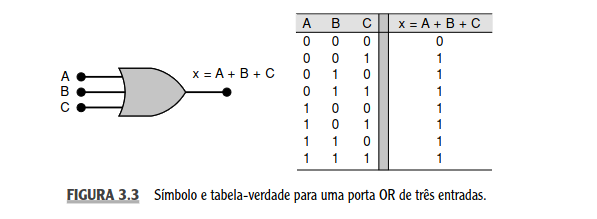
\includegraphics[width=\textwidth]{Figuras/Ou-2.png}

    \end{figure}

\end{frame}

\begin{frame}{A Porta OR em Circuitos Digitais}
    \begin{itemize}
        \item \textbf{Definição:} Circuito com duas ou mais entradas cuja saída é o resultado da combinação das entradas via operação OR.
        \item \textbf{Níveis Lógicos:} As entradas (A, B) e a saída ($x$) são representadas por níveis lógicos de tensão.
        \item \textbf{Símbolo Lógico:} Possui representação específica para indicar a operação $x = A + B$.
    \end{itemize}
\end{frame}

\begin{frame}{Lógica de Operação da Porta OR}
    \begin{itemize}
        \item \textbf{Saída ALTA (1):} Ocorre se a entrada A, ou a entrada B, ou ambas forem nível lógico 1.
        \item \textbf{Saída BAIXA (0):} Ocorre apenas se \textbf{todas} as entradas forem nível lógico 0.
        \item \textbf{Resumo:} Basta que uma única entrada esteja em nível 1 para que a saída também seja 1.
    \end{itemize}
\end{frame}

\begin{frame}{Múltiplas Entradas}
    \begin{itemize}
        \item \textbf{Extensibilidade:} O princípio aplica-se a portas OR com qualquer número de entradas (ex: 3 entradas).
        \item \textbf{Expressão Booleana:} Para três entradas, a saída é expressa como $x = A + B + C$.
        \item \textbf{Notação:} O sinal $+$ reforça o uso da operação lógica OR entre as várias entradas.
        \item \textbf{Tabela-Verdade:} Confirma que a saída será 1 em todos os casos onde houver uma ou mais entradas em 1.
    \end{itemize}
\end{frame}

\begin{frame}{OU com 3 entradas}

    \begin{figure}
        \centering

        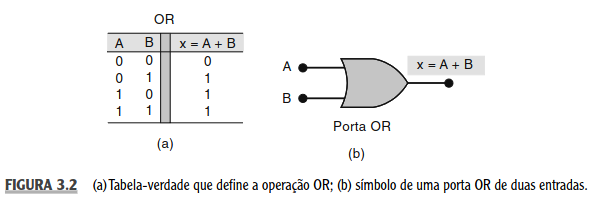
\includegraphics[width=\textwidth]{Figuras/Ou-1.png}

    \end{figure}

\end{frame}

\begin{frame}{Resumo da Operação OR}
    \begin{itemize}
        \item \textbf{Regra Fundamental:} A operação OR gera um resultado (saída) \textbf{1} sempre que quaisquer das entradas for \textbf{1}. Caso contrário, a saída é \textbf{0}.
        \item \textbf{Definição de Porta OR:} É o circuito lógico que realiza fisicamente a operação OR sobre as entradas aplicadas.
        \item \textbf{Leitura da Expressão:} A equação $x = A + B$ deve ser lida como: \textit{“x é igual a A ou B”}.
    \end{itemize}
\end{frame}

\begin{frame}{Exemplo Prático: Operação OR}
    \textbf{Frase:} "Vou à praia se for Sábado (A) OU se estiver Ensolarado (B)"
    \vspace{0.4cm}
    \begin{itemize}
        \item \textbf{A = 1:} É sábado | \textbf{A = 0:} Não é sábado
        \item \textbf{B = 1:} Tem sol | \textbf{B = 0:} Não tem sol
    \end{itemize}
    \vspace{0.2cm}
    \begin{table}
        \centering
        \begin{tabular}{|c|c||c|}
            \hline
            \textbf{A (Sábado)} & \textbf{B (Sol)} & \textbf{x (Praia)} \\ \hline
            0                   & 0                & 0                  \\ \hline
            0                   & 1                & 1                  \\ \hline
            1                   & 0                & 1                  \\ \hline
            1                   & 1                & 1                  \\ \hline
        \end{tabular}
    \end{table}
\end{frame}

\begin{frame}{Operação OR com 3 Entradas}
    \textbf{Exemplo Prático:} ``Eu vou ao parque se for Sábado (A) OU se tiver Sol (B) OU se eu ganhar uma carona (C).''
    \vspace{0.4cm}
    \begin{itemize}
        \item \textbf{Entradas (Variáveis):}
              \begin{itemize}
                  \item $A$: É sábado ($1=$ sim, $0=$ não)
                  \item $B$: Está sol ($1=$ sim, $0=$ não)
                  \item $C$: Ganhei carona ($1=$ sim, $0=$ não)
              \end{itemize}
        \item \textbf{Expressão Booleana:} $x = A + B + C$
        \item \textbf{Lógica:} A saída $x$ é 1 se $A$ ou $B$ ou $C$ (ou qualquer combinação deles) for 1.
    \end{itemize}
\end{frame}

\begin{frame}{Tabela-Verdade: 3 Entradas ($2^3 = 8$ linhas)}
    \begin{table}
        \centering
        \small
        \begin{tabular}{|c|c|c||c|}
            \hline
            \textbf{A (Sábado)} & \textbf{B (Sol)} & \textbf{C (Carona)} & \textbf{x (Parque)} \\ \hline
            0                   & 0                & 0                   & \textbf{0}          \\ \hline
            0                   & 0                & 1                   & \textbf{1}          \\ \hline
            0                   & 1                & 0                   & \textbf{1}          \\ \hline
            0                   & 1                & 1                   & \textbf{1}          \\ \hline
            1                   & 0                & 0                   & \textbf{1}          \\ \hline
            1                   & 0                & 1                   & \textbf{1}          \\ \hline
            1                   & 1                & 0                   & \textbf{1}          \\ \hline
            1                   & 1                & 1                   & \textbf{1}          \\ \hline
        \end{tabular}
    \end{table}
    \vspace{0.2cm}
    \centering
    \textit{A saída é 0 apenas quando todas as entradas são 0 simultaneamente.}
\end{frame}

\begin{frame}{Porta OR de 3 Entradas}
    \begin{itemize}
        \item \textbf{Símbolo:} O símbolo possui três terminais de entrada e um de saída.
        \item \textbf{Funcionamento:} Opera de modo que a saída será ALTA (1) se qualquer entrada for ALTA.
        \item \textbf{Soma Booleana:} $1 + 1 + 1 = 1$. O resultado nunca ultrapassa o nível lógico 1.
    \end{itemize}
    \vspace{0.5cm}
    \begin{center}

    \end{center}
\end{frame}

\begin{frame}{Operação AND (E)}
    \begin{itemize}


        \item \textbf{Regra de Saída:} A saída $x$ será nível lógico 1 \textbf{apenas} quando todas as entradas forem 1.
        \item \textbf{Caso de Nível 0:} Se qualquer uma das entradas for 0, a saída será obrigatoriamente 0.
    \end{itemize}
\end{frame}

\begin{frame}{Expressão Booleana e Notação}
    \begin{itemize}
        \item \textbf{Equação:} $x = A \cdot B$ ou simplesmente $x = AB$.
        \item \textbf{O Sinal ($\cdot$):} Representa a operação booleana AND.
        \item \textbf{Relação com a Multiplicação:}
              \begin{itemize}
                  \item A operação AND equivale à multiplicação convencional entre variáveis booleanas ($0 \cdot 0 = 0$; $0 \cdot 1 = 0$; $1 \cdot 1 = 1$).
              \end{itemize}
        \item \textbf{Leitura:} “$x$ é igual a $A$ e $B$”.
    \end{itemize}
\end{frame}

\begin{frame}{Múltiplas Entradas na Operação AND}
    \begin{itemize}
        \item \textbf{Três entradas:} $x = A \cdot B \cdot C = ABC$.
        \item \textbf{Leitura:} “$x$ é igual a $A$ e $B$ e $C$”.
        \item \textbf{Condição de saída 1:} $x$ será 1 \textbf{apenas} quando as variáveis $A, B$ e $C$ forem, simultaneamente, nível 1.
        \item \textbf{Exemplo:} Se qualquer entrada for 0, o produto lógico resulta em 0.
    \end{itemize}
\end{frame}

\begin{frame}{Tabela-Verdade da Operação AND}
    Resumo das combinações para duas entradas:
    \vspace{0.2cm}
    \begin{table}
        \centering
        \begin{tabular}{cc|c}
            \hline
            \textbf{A} & \textbf{B} & \textbf{x = AB} \\ \hline
            0          & 0          & 0               \\
            0          & 1          & 0               \\
            1          & 0          & 0               \\
            1          & 1          & 1               \\ \hline
        \end{tabular}
    \end{table}
\end{frame}

\begin{frame}{E com 2 entradas}

    \begin{figure}
        \centering

        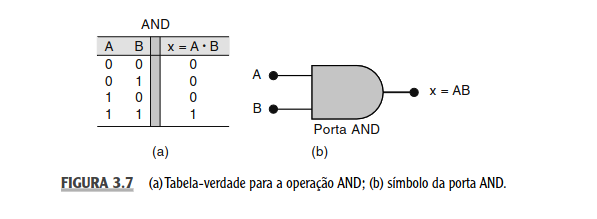
\includegraphics[width=\textwidth]{Figuras/and-1.png}

    \end{figure}

\end{frame}

\begin{frame}{A Porta AND em Circuitos Digitais}
    \begin{itemize}
        \item \textbf{Definição:} Circuito que opera de modo que sua saída seja nível ALTO \textbf{somente} quando todas as entradas também o forem.
        \item \textbf{Expressão de Saída:} A saída é igual ao produto lógico das entradas: $x = AB$.
        \item \textbf{Estados de Operação:}
              \begin{itemize}
                  \item Para todos os outros casos (onde houver pelo menos um zero), a saída será nível BAIXO (0).
              \end{itemize}
    \end{itemize}
\end{frame}

\begin{frame}{Múltiplas Entradas e Símbolos}
    \begin{itemize}
        \item \textbf{Extensibilidade:} O princípio é o mesmo para qualquer número de entradas.
        \item \textbf{Exemplos:}
              \begin{itemize}
                  \item Porta de 3 entradas: $x = ABC$.
                  \item Porta de 4 entradas: $x = ABCD$.
              \end{itemize}
        \item \textbf{Consistência:} A saída será 1 apenas no caso em que todas as entradas ($A = B = C = \dots = 1$) sejam 1.
    \end{itemize}
    \vspace{0.3cm}
    \begin{center}

    \end{center}
\end{frame}

\begin{frame}{E com 3 entradas}

    \begin{figure}
        \centering

        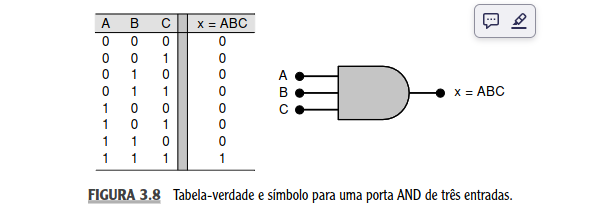
\includegraphics[width=\textwidth]{Figuras/and-2.png}

    \end{figure}

\end{frame}


\begin{frame}{Exemplo Prático: Operação AND (2 Entradas)}
    \textbf{Frase:} ``Eu só vou à praia se for Sábado \textbf{E} se estiver Ensolarado.''
    \vspace{0.4cm}
    \begin{itemize}
        \item \textbf{A:} É sábado ($1 = $ Sim | $0 = $ Não)
        \item \textbf{B:} Está ensolarado ($1 = $ Sim | $0 = $ Não)
        \item \textbf{x:} Vou à praia ($x = A \cdot B$)
    \end{itemize}
    \vspace{0.2cm}
    \begin{table}
        \centering
        \begin{tabular}{|c|c||c|l|}
            \hline
            \textbf{A} & \textbf{B} & \textbf{x} & \textbf{Cenário}                             \\ \hline
            0          & 0          & \textbf{0} & Não é sábado e chove. (Fico em casa)         \\ \hline
            0          & 1          & \textbf{0} & Tem sol, mas é dia de semana. (Fico em casa) \\ \hline
            1          & 0          & \textbf{0} & É sábado, mas está chovendo. (Fico em casa)  \\ \hline
            1          & 1          & \textbf{1} & É sábado \textbf{E} tem sol. (Vou à praia!)  \\ \hline
        \end{tabular}
    \end{table}
\end{frame}

\begin{frame}{Exemplo Prático: Operação AND (3 Entradas)}
    \textbf{Frase:} ``Eu só vou ao parque se for Sábado (A) \textbf{E} tiver Sol (B) \textbf{E} eu ganhar Carona (C).''
    \vspace{0.4cm}
    \begin{itemize}
        \item \textbf{Expressão:} $x = A \cdot B \cdot C$ (ou $x = ABC$)
    \end{itemize}
    \vspace{0.2cm}
    \begin{table}
        \centering
        \small
        \begin{tabular}{|c|c|c||c|}
            \hline
            \textbf{A (Sábado)} & \textbf{B (Sol)} & \textbf{C (Carona)} & \textbf{x (Parque)} \\ \hline
            0                   & 0                & 0                   & \textbf{0}          \\ \hline
            0                   & 1                & 1                   & \textbf{0}          \\ \hline
            1                   & 0                & 1                   & \textbf{0}          \\ \hline
            1                   & 1                & 0                   & \textbf{0}          \\ \hline
            1                   & 1                & 1                   & \textbf{1}          \\ \hline
        \end{tabular}
    \end{table}
    \vspace{0.2cm}
    \begin{block}{Observação}
        Diferente do OR, aqui a saída é \textbf{0} na maioria dos casos. O resultado só é \textbf{1} quando todas as entradas são verdadeiras simultaneamente.
    \end{block}
\end{frame}

\begin{frame}{Resumo da Operação AND}
    \begin{itemize}
        \item \textbf{Aritmética:} A operação AND é realizada da mesma maneira que a multiplicação convencional de 1s e 0s.
        \item \textbf{Circuito:} Uma porta AND é um circuito lógico que realiza fisicamente a operação AND sobre as entradas do circuito.
        \item \textbf{Regra de Saída:} A saída de uma porta AND será \textbf{1 somente quando todas as entradas forem 1}; para todos os outros casos, a saída será \textbf{0}.
        \item \textbf{Leitura:} A expressão $x = AB$ deve ser lida como: \textit{“x é igual a A e B”}.
    \end{itemize}
    \vspace{0.4cm}
    \begin{block}{Comparação de Saída}
        \centering
        \begin{tabular}{c|c}
            \textbf{Condição de Entrada} & \textbf{Resultado AND} \\ \hline
            Qualquer entrada é 0         & Saída = 0              \\
            Todas as entradas são 1      & Saída = 1              \\
        \end{tabular}
    \end{block}
\end{frame}


\begin{frame}{Diferenciação: Porta AND vs. Porta OR}
    É fundamental observar a diferença entre os símbolos e comportamentos:
    \vspace{0.4cm}
    \begin{itemize}
        \item \textbf{Símbolo AND:} Indica que a saída será nível ALTO \textbf{somente} quando todas as entradas forem nível ALTO.
        \item \textbf{Símbolo OR:} Indica que a saída será nível ALTO quando \textbf{qualquer} entrada for nível ALTO.
    \end{itemize}
    \vspace{0.4cm}
    \begin{block}{Regra Prática}
        Em um diagrama de circuito, a porta AND exige totalidade de sinais altos, enquanto a porta OR exige apenas uma presença.
    \end{block}
\end{frame}

\begin{frame}{Operação NOT (Inversão)}
    \begin{itemize}
        \item \textbf{Diferencial:} Realizada sobre uma \textbf{única variável} de entrada (diferente de OR e AND).
        \item \textbf{Expressão Booleana:} $x = \bar{A}$
        \item \textbf{Leituras:}
              \begin{itemize}
                  \item $x$ é igual a $A$ negado.
                  \item $x$ é igual ao inverso de $A$.
                  \item $x$ é igual ao complemento de $A$.
              \end{itemize}
        \item \textbf{Conceito:} O valor lógico de saída é o oposto do valor lógico de $A$.
    \end{itemize}
\end{frame}

\begin{frame}{Tabela-Verdade e Notação}
    \begin{columns}
        \begin{column}{0.5\textwidth}
            \begin{table}
                \centering
                \begin{tabular}{|c|c|}
                    \hline
                    \textbf{A} & \textbf{x = $\bar{A}$} \\ \hline
                    0          & 1                      \\ \hline
                    1          & 0                      \\ \hline
                \end{tabular}
            \end{table}
        \end{column}
        \begin{column}{0.5\textwidth}
            \begin{itemize}
                \item $\bar{0} = 1$ (0 é 1 NEGADO).
                \item $\bar{1} = 0$ (1 é 0 NEGADO).
            \end{itemize}
        \end{column}
    \end{columns}
    \vspace{0.4cm}
    \textbf{Indicadores de Inversão:}
    \begin{itemize}
        \item Barra sobre a variável ($\bar{A}$).
        \item Apóstrofo ($A'$).
    \end{itemize}
\end{frame}

\begin{frame}{Circuito NOT (INVERSOR)}
    \begin{itemize}
        \item \textbf{Definição:} Mais comumente denominado \textbf{INVERSOR}.
        \item \textbf{Características:}
              \begin{itemize}
                  \item Tem sempre apenas uma entrada.
                  \item O nível lógico de saída é o oposto ao nível de entrada.
              \end{itemize}
        \item \textbf{Efeito no Sinal:} Inverte (complementa) o sinal de entrada em todos os pontos da forma de onda.
        \item \textbf{Resumo:} Se entrada = 0, saída = 1; se entrada = 1, saída = 0.
    \end{itemize}
    \vspace{0.3cm}
    \begin{center}
        % [Símbolo lógico e forma de onda seriam inseridos aqui conforme Figura 3.11]
    \end{center}
\end{frame}

\begin{frame}{Operacao NOT}

    \begin{figure}
        \centering

        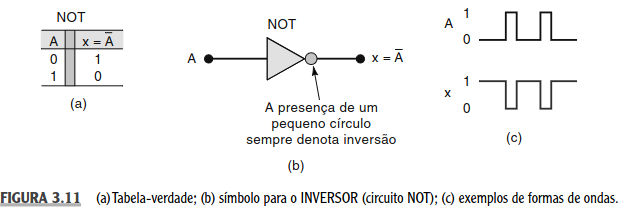
\includegraphics[width=\textwidth]{Figuras/not-1.png}

    \end{figure}

\end{frame}

\begin{frame}{Comparação OR AND NOT}

    \begin{figure}
        \centering

        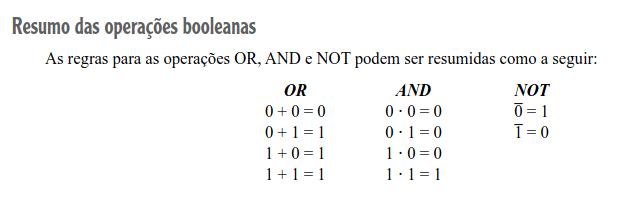
\includegraphics[width=\textwidth]{Figuras/resumo-or-and-not.png}

    \end{figure}

\end{frame}

\begin{frame}{Circuito Exclusive-OR (XOR)}
    \begin{itemize}
        \item \textbf{Definição:} Circuito que produz uma saída em nível ALTO sempre que as duas entradas estiverem em \textbf{níveis opostos}.
        \item \textbf{Abreviação:} XOR.
        \item \textbf{Porta Lógica:} Devido à sua utilidade e frequência de uso, possui um símbolo próprio e é considerada um tipo de porta lógica.
        \item \textbf{Restrição:} Uma porta XOR tem apenas duas entradas; não existem portas XOR de três ou quatro entradas.
    \end{itemize}
\end{frame}

\begin{frame}{Expressão Lógica e Notação}
    \begin{itemize}

        \item \textbf{Forma Abreviada:}
              $$x = A \oplus B$$
        \item \textbf{Operação:} O símbolo $\oplus$ representa a operação da porta XOR.
    \end{itemize}
\end{frame}

\begin{frame}{Tabela-Verdade da Porta XOR}
    \begin{table}
        \centering
        \begin{tabular}{|c|c||c|}
            \hline
            \textbf{A} & \textbf{B} & \textbf{x} \\ \hline
            0          & 0          & 0          \\ \hline
            0          & 1          & 1          \\ \hline
            1          & 0          & 1          \\ \hline
            1          & 1          & 0          \\ \hline
        \end{tabular}
        \caption{Tabela-verdade para $x = A \oplus B$}
    \end{table}
\end{frame}

\begin{frame}{Características Resumidas da Porta XOR}
    \begin{enumerate}
        \item Tem apenas duas entradas.
        \item Expressão de saída: $A \oplus B$.
        \item A saída será nível ALTO \textbf{apenas} quando as duas entradas estiverem em níveis diferentes.
    \end{enumerate}
    \vspace{0.5cm}

\end{frame}


\begin{frame}{XOR - Ou Exclusivo}

    \begin{figure}
        \centering

        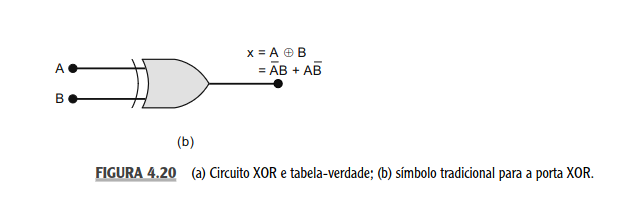
\includegraphics[width=\textwidth]{Figuras/xor-1.png}

    \end{figure}

\end{frame}